
\section*{Exercise 3}
\label{sec:exercise-3}

\subsection*{(a)}
\label{sec:a-2}
The plot of the profiles are presented in figure
\ref{fig:ex3-profiles}.
\begin{figure}[h]
  \centering
  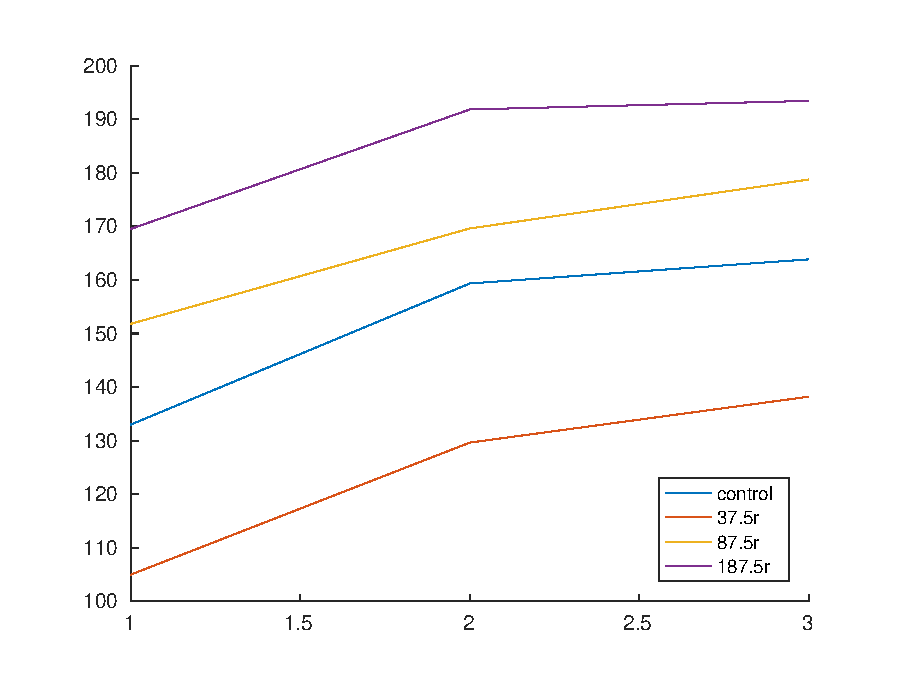
\includegraphics[width=8.5cm]{ex3-profiles}
  \caption{The profiles for the Psychmotor scores given different
    radiation treatment.}
  \label{fig:ex3-profiles}
\end{figure}

\subsection*{(b)}
\label{sec:b-2}


Since we have more than tho profiles we wich to test, we have to use
the more general approach. Set up the variables as descibed in Lectrure
6. We can test if the profiles are parallel using
\begin{equation*}
  \lambda_{H_1} = \frac{\det CVC^T}{\det( CVC^T  + CHC^T),}
\end{equation*}
and createing the test variables
\begin{equation*}
  test = -\left(n - \frac 12(k + p -1)\right) \ln \Lambda_{H_1},
\end{equation*}
which is $\chi^2((p-1)(k-1))$. We reject $H_1$ if test variable is
smaller then the critical point, 
\begin{equation*}
  c = \chi^2 _{0.95} ((p-1)(k-1)).
\end{equation*}
From matlab we get
\begin{equation*}
  test = -4.0443,
\end{equation*}
and
\begin{equation*}
    c = 12.5916.
\end{equation*}
Since we $test < c$, we can not reject $H_1$, the profiles are parallel.


\subsection*{(c)}
\label{sec:c-2}

Since, the profiles are parallel, we can set up a test for checking if
the profiles are on the same level. This can be done by using the test
\begin{equation*}
  \lambda_{H_2 | H_1} = \frac{\det(CVC^T + CHC^T)}{\det(CVC^T)}\frac{\det(V)}{\det(V+H)},
\end{equation*}
and creating the test variable 
\begin{equation*}
  F = \left(\frac{n-k - p +1}{k - 1}\right)\frac{1 - \lambda_{H_2 |H_1}}{\lambda_{H_2 | H_1}},
\end{equation*}
which we compare to the critical value
\begin{equation*}
  c = F_{0.95} (k-1, n - k - p +1).
\end{equation*}
We get
\begin{equation*}
  -10.8296 = F < c = 2.8451,
\end{equation*}
we can not reject $H_2 | H_1$, the profiles are on the same level.

\subsection*{(d)}
\label{sec:d-1}

Here, we use the test variables 
\begin{equation*}
  \lambda_{H_3 | H_1} = \frac{1}{1 + n \bar{\bf x}^T C^T (CVC^T +
    CHC^T)^-1C*\bar{\bf x}},
\end{equation*}
and create the test variable
\begin{equation*}
  test = \frac{n - p +1}{p - 1}\lambda_{H_3 |H_1},
\end{equation*}
which we compare to 
\begin{equation*}
  c = F_{0.95}(p-1, n-p+1).
\end{equation*}
We get
\begin{equation*}
  7.9361 = test > c = 3.2145.
\end{equation*}
So we get that we have to reject $H_3 | H_1$, the profiles are not
flat.

\section*{\texttt{matlab} code}
\label{sec:textttmatlab-code}

\lstinputlisting[style=matlab]{../ex3.m}
%%% Local Variables:
%%% mode: latex
%%% TeX-master: "examination"
%%% End:
